\documentclass{article}
\usepackage{stmaryrd}
\usepackage{url}

\title{Project report: Coupling ScimBa and Feel++}

\author{Helya Amiri, Rayen Tlili}
\date{}

\begin{document}

\maketitle

\tableofcontents
\newpage


\section{Introduction}

This report presents the objectives, approach, and roadmap for the coupling of ScimBa and Feel++ libraries. ScimBa is a project aimed at integrating machine learning techniques with traditional scientific computing methods, while Feel++ is a C++ implementation of Galerkin methods for solving partial differential equations (PDEs). The coupling of these two libraries is expected to enhance their capabilities and enable researchers to solve complex scientific problems more effectively.



\subsection{Objectives}

This project seeks to facilitate the coupling of ScimBa and Feel++.
The primary objective is to establish loose coupling between ScimBa and Feel++, enabling efficient utilization of their respective strengths.

\subsection{Roadmap}
\begin{frame}{Github Roadmap}
    \begin{center}
        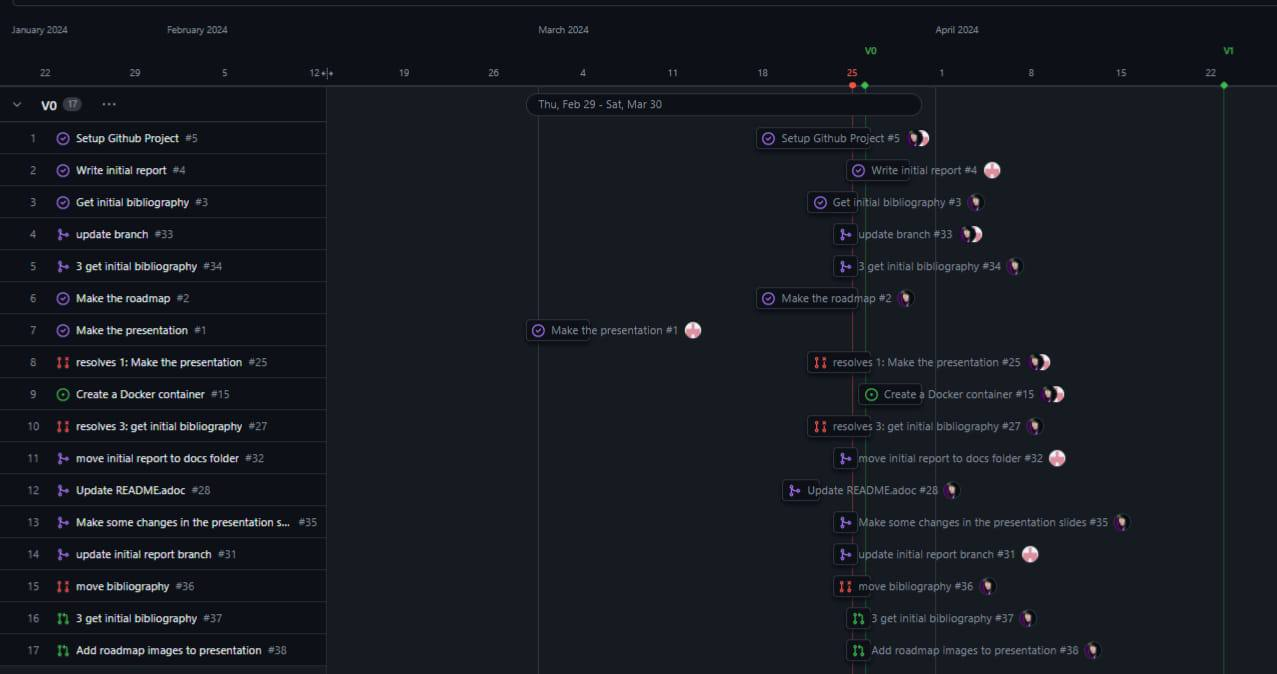
\includegraphics[width=0.7\textwidth]{images/roadmap1.png}
        \vspace{1em} % Ajoute un espace vertical
        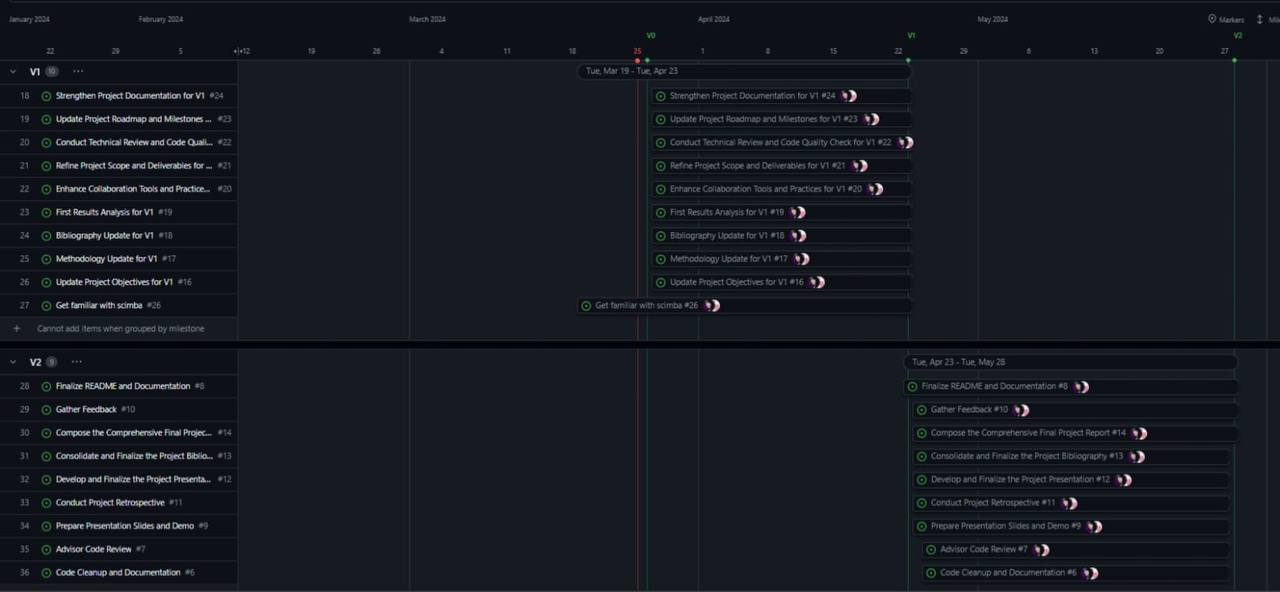
\includegraphics[width=0.7\textwidth]{images/roadmap2.png}
    \end{center}
\end{frame}

The general outline as of the start of the project includes the following goals:

\begin{enumerate}
    \item \textbf{Analysis and Planning:} Analyze the functionalities of ScimBa and Feel++ to identify integration points. Develop a plan for implementing loose coupling between the two libraries.
    \item \textbf{Implementation:} Implement loose coupling between ScimBa and Feel++ according to the planned approach. Develop methods for generating datasets using Feel++ and integrating them into ScimBa.
    \item \textbf{Testing and Validation:} Test the integrated system to ensure that communication between ScimBa and Feel++ is seamless. Validate the effectiveness of the coupling by solving complex scientific problems.
    \item \textbf{Documentation and Reporting:} Document the integration process, including interface definitions and communication protocols. Prepare a final report summarizing the project outcomes and lessons learned.
\end{enumerate}

\section{Getting started}
\subsection{Creating a Docker container}
Creating a Docker container and image for the project offers these key advantages:
\begin{enumerate}
 \item \textbf{Portability:} Run the project on any platform supporting Docker.
 \item \textbf{Isolation:} Avoid conflicts with other software on the host system.
 \item \textbf{Reproducibility:} Recreate the exact same environment whenever needed.
 \item \textbf{Dependency Management:} Package all dependencies within the Docker image.


\end{enumerate}
We're using Feel++ as the base for the Docker container adding the requirements and dependencies for Scimba.

This contains the latest version of Feel++ and Scimba and should be able to run these commands without error:

\begin{verbatim}
python
import feelpp
import scimba
\end{verbatim}

\begin{frame}{Dockerfile}
    \begin{center}
        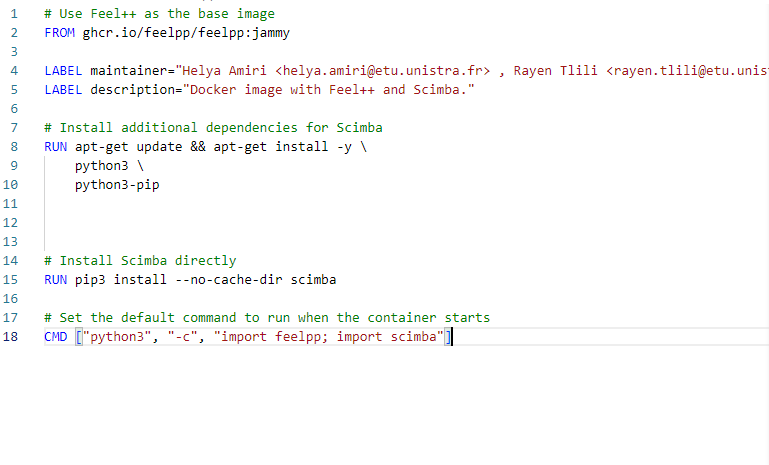
\includegraphics[width=0.7\textwidth]{images/dockerfile.png}
    \end{center}
\end{frame}

\subsection{Exploring Feel++ toolboxes}

As of the first meeting with the project supervisors, we've taken a look at the different toolboxes Feel++ has to offer in python:

\begin{frame}{}
    \begin{center}
        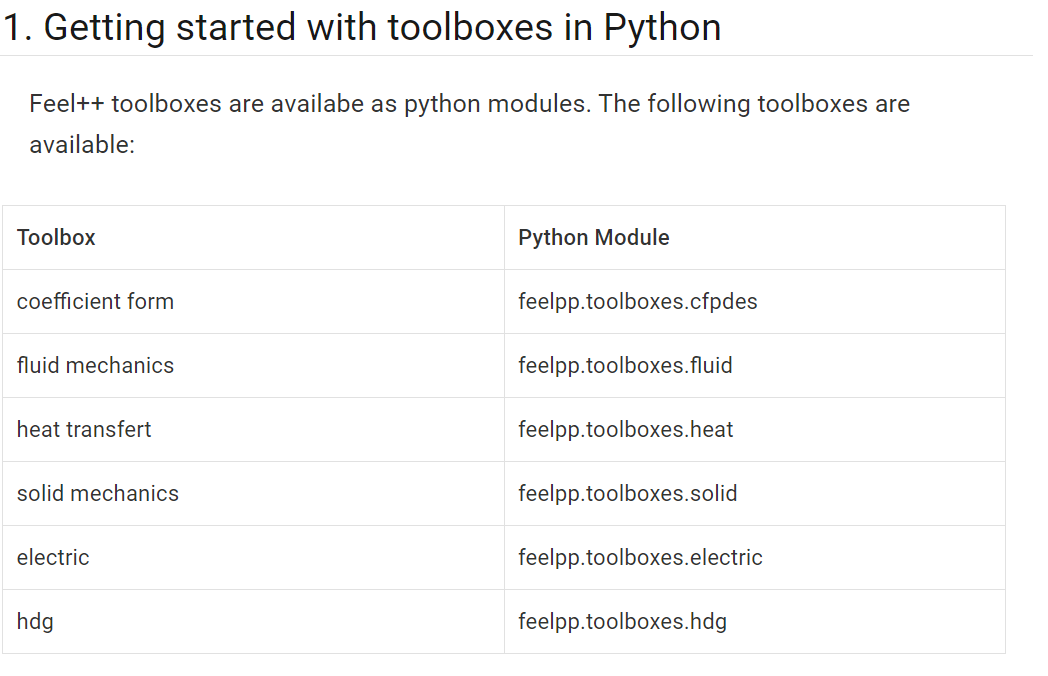
\includegraphics[width=0.7\textwidth]{images/pyfeelpptoolboxes.png}
    \end{center}
\end{frame}

An interesting toolbox to start with is the \textbf{Coefficient Form PDEs}.

\begin{frame}{}
    \begin{center}
        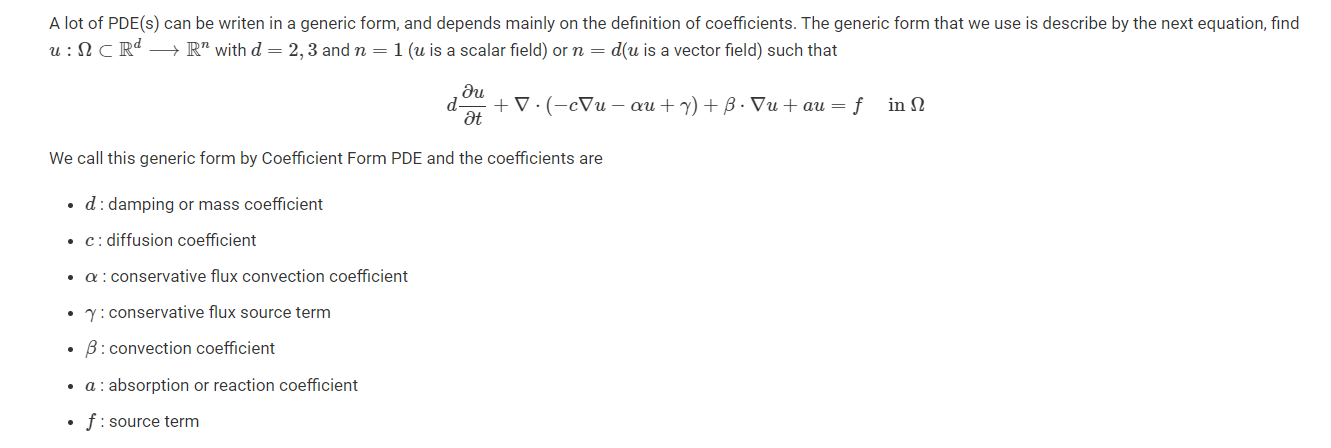
\includegraphics[width=0.7\textwidth]{images/cfpde.png}
    \end{center}
\end{frame}

\begin{frame}{}

This toolbox allows users to solve PDEs in a generic manner just by inputting the different coefficient values. Implementing an interface which, through Scimba, calls Feel++, solves the PDE and retrieves the solution would be very powerful as it enables us to approach solving for Laplacian and heat transfer problems for example.
\end{frame}




\section{Bibliography}

\begin{itemize}
    \item Feel++ Documentation: \url{https://docs.feelpp.org/user/latest/index.html}
    \item ScimBa Documentation: \url{https://sciml.gitlabpages.inria.fr/scimba/}
    \item Coupling (Computer Programming): \url{https://en.wikipedia.org/wiki/Coupling_(computer_programming)}
    \item Using feel++:
    \url{https://www.cemosis.fr/events/course-solving-pdes-with-feel/}
\end{itemize}

\end{document}
